%\section{Physical Human Factors Report: Tristan Griffith}
\rhead{\today}
\begin{center}
{\large  Tristan Griffith}\\
\vspace{2mm}
{\large Dr. James Hubbard Jr.}
\noindent\rule{\textwidth}{2pt}
\end{center}
\setcounter{section}{1}

%\begin{wrapfigure}{r}{0.45\textwidth}
%\centering
%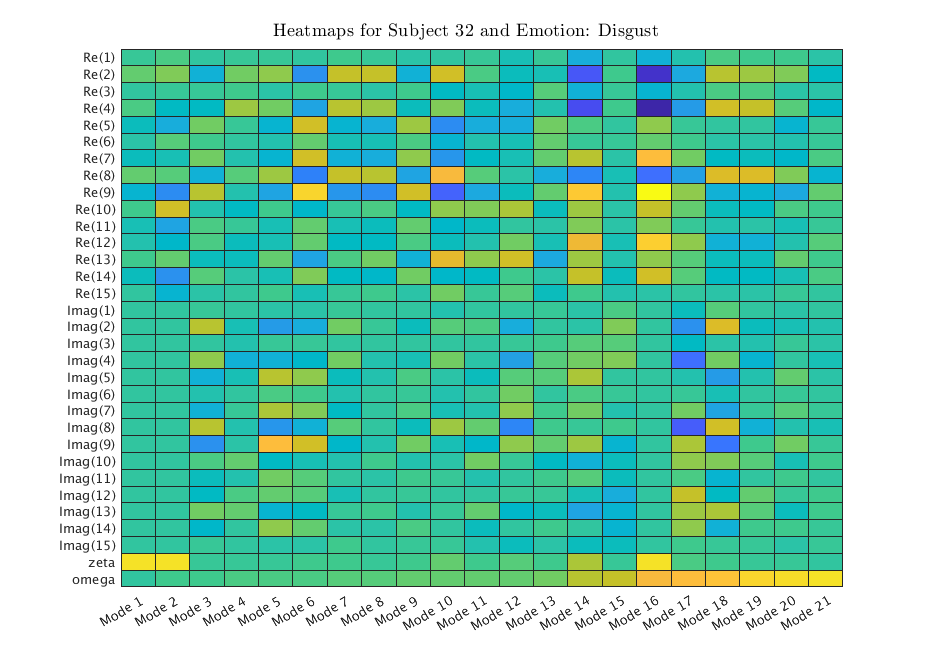
\includegraphics[scale=.3]{../../../figures/demo_map.png} 
%\caption{Modal Heatmap for Subject 32}
%\end{wrapfigure}
\subsection{Introduction}
We inquire concerning the nature of traveling waves in the brain. Under this head there are three points of inquiry:
\begin{enumerate}
\item Whether the brain has traveling waves?
\item Whether fMRI waves are connected to EEG waves?
\item If traveling waves exist, are they relevant to clinical outcomes?
\end{enumerate}
\subsection{Whether the brain has traveling waves?}
\textbf{Keyword differences:} First, note that the notion of a traveling wave is different for neuroscience and engineering. Neuroscientists would denote any brain wave that is observable across the sensor locations as a traveling wave. Engineers reserve traveling wave for behavior which is not in phase across the spatial sensors. In phase behavior is called a standing wave, while out of phase is a traveling wave. Neuroscientists would call both traveling waves. Going forward, I will use traveling wave in the engineering sense, denoting standing waves where needed. \\
\textbf{Objection 1:} Prior work has shown repeated decoherence among spatially distributed recordings of brain activity. Theta oscillations in humans are postulated to have only local mechanisms \cite{doi:10.1152/jn.00409.2005}. 
\begin{displayquote}
 We found that, whereas nearby gated sites $(<20 \textit{mm})$ were often but not always coherent, distant gated sites were almost never coherent. Our results imply that there are local mechanisms for the generation of cortical theta.
\end{displayquote}
\textbf{Objection 2:} While inter-electrode spatial correlations in the gamma band have been discovered in animals, the same was not found in humans \cite{MENON199689}.
\begin{displayquote}
The findings suggest that the surface diameters of domains of spatially correlated activity underlying perceptual categorization in human gamma band ECoG are limited to less than 2 cm and that the intermittent synchronization observed across separations of 1 cm and 1.4 cm is not solely due to volume conduction. Thus, if such gamma band spatial patterns exist in the human brain, no existing technology would be capable of measuring them at the scalp, and subdural electrode arrays for cortical surface recording would have to have spacings under 5 mm.
\end{displayquote}
\textbf{Objection 3:} Using statistical methods, EEG coherence was found to decline substantially in space across all frequency bands \cite{BULLOCK1995161}.
\begin{displayquote}
In both the subdural surface samples and those from temporal lobe depth electrode arrays coherent declines with distance between electrodes of the pair, on the average quite severely in millimeters. This is nearly the same for all frequency bands. 
\end{displayquote}
\textbf{On the contrary,} it has been found most recently that when \textbf{phase} is considered as part of the spatial coherence, traveling and standing waves are observed across a broad spectrum for most subjects \cite{ZHANG20181269}.\\

I argue that, in each of the objections above, the possibility of complex traveling waves was ignored. In each of these studies, it was assumed that the spatial activity of the brain's electrical activity would be described by perfect sine and cosine waves in two dimensions. This excludes the possibility of damping in the oscillatory behavior of the electrical activity. Many mechanical systems have damping, so why should we exclude this possibility in the analysis of the brain? To this end, our output only modal analysis has shown significant spatial dependence when both proportional and non-proportional damping is considered. Unlike the objections above, the naiveté of our engineering first approach is a strength, because it does not exclude the possibility of complex eigenmodes. Further, studies \cite{doi:10.1152/jn.00409.2005} and \cite{BULLOCK1995161} argue that low correlation of the band power is sufficient evidence to exclude the possibility of spatial dependence in the activity of the brain. I argue that a single, simple statistical tool is not sufficient proof for such a broad claim. There is no consideration of phase or damping.  Ultimately, we discovered that 20\% of the eigenmodes are damped on average, with 50\% showing some out of phase behavior. At present this issue is \textbf{closed.}
\subsection{Whether fMRI waves are connected to EEG waves?}
\textbf{Objection 1:} Using band power and statistical tests, EEG and fMRI were found to be inversely correlated on average, but not significantly enough to report \cite{LAUFS20031463}:
\begin{displayquote}
A more general problem is that our current understanding of EEG and fMRI (or PET) signals does not allow us to extrapolate whether and, if so, how the oscillatory synchronization of electrical synaptic activity in the alpha band translates into hemodynamic signals. The mere fact that synaptic activity takes on the temporal structure of an oscillation does not mean that net synaptic activity changes over time, and the oscillation frequencies of physiological rhythms themselves are beyond the temporal resolution of hemodynamic signals.
\end{displayquote}
\textbf{Objection 2:} In a comprehensive survey, \cite{SALEKHADDADI2003110} reports that despite improvements in sensing technology, disparate studies considering many different hypotheses have been unable to realize a unified connection between fMRI and EEG. Questions even arise concerning the nature of spontaneous EEG (e.g. is the rest state actually a rest state?). Because it is difficult to define consistent operating conditions from subject to subject a connection between fMRI and EEG is non-trivia:
\begin{displayquote}
We have reviewed the existing literature on this topic and have explored both the theoretical and practical limitations of EEG/fMRI with specific emphasis on studying the generators of IEDs. We envisage that further characterization of the BOLD correlates of spontaneous EEG activity and the development of ever more sophisticated fMRI models will constitute a significant effort over the next few years.
\end{displayquote}
\textbf{Further,} A despite a great amount of effort, experimental and theoretical work has been unable to explain the link between EEG and BOLD signals, as discussed in \cite{10.3389/fneur.2013.00001}:
\begin{displayquote}
The most consensual evidence comes from the recording of electrical activity using micro-electrodes implanted in the cortex of (non-human) animals, simultaneously with fMRI, indicating that the BOLD signal reflects mostly slow, post-synaptic input activity measured by local field potentials (LFPs), rather than fast, spiking output activity measured by single/multi-unit activity (S/MUA; Logothetis et al., 2001). In humans, a growing number of simultaneous EEG-fMRI studies on healthy subjects as well as epilepsy patients have now been reported (Goldman et al., 2002; Laufs et al., 2003, 2006; Moosmann et al., 2003; de Munck et al., 2009), and biophysical models of the neurovascular coupling have been proposed (Riera et al., 2006, 2007). Overall, reports in the literature do not provide a clear picture of the link between EEG and BOLD signals. In particular, contradictory results have been presented regarding the dependency of BOLD changes on the EEG power and spectral profiles. These include, for example, positive and negative BOLD correlations with specific frequency band power changes in the human EEG (de Munck et al., 2009), BOLD decoupling from LFP power in mice (Ekstrom, 2010), and negative BOLD associated with large increases in LFP and MUA during seizures also in mice (Schridde et al., 2008). Rosa et al. (2010b) addressed this topic by comparing different models of the transfer function between EEG and BOLD signals, in the prediction of fMRI data, in a visual stimulation experiment with human healthy subjects. The models explored included the EEG total power (TP; Wan et al., 2006); linear combinations of the power from different frequency bands (Goense and Logothetis, 2008); and several variations of a heuristic model proposed by Kilner et al. (2005) in which BOLD changes are assumed to be proportional to the root mean square frequency (RMSF) of the EEG spectrum. The results obtained showed a clear superiority of the RMSF metrics in predicting the BOLD signal, when compared to power-weighted metrics.
\end{displayquote}
\textbf{At present,} I argue that our modal decomposition method offers a compelling spatial representation of the data which may be more easily compared with a BOLD time series. \textcolor{red}{I estimate it would take approximately 3 weeks to process a data set with EEG and fMRI signals in order to compare the modes.} We have seen some empirical evidence that the shapes are similar, but more work is needed to verify frequencies and mode shapes are significant. At present this issue is \textbf{\textcolor{red}{open}} in both our work and the broader literature.

\subsection{If traveling waves exist, are they relevant to clinical outcomes?}
\textbf{Objection 1:} \cite{Massimini6862} found that while a standing wave was present during sleep, there was not enough evidence to say if it was a function of the cognitive state or the natural resting state of the brain.
\begin{displayquote}
The pattern of origin and propagation of sleep slow oscillations is reproducible across nights and subjects and provides a blueprint of cortical excitability and connectivity. The orderly propagation of correlated activity along connected pathways may play a role in spike timing-dependent synaptic plasticity during sleep.
\end{displayquote}
\textbf{Objection 2:} \cite{Takahashi0} found that as in animal brains, there are standing waves in human brains that propagate 180\degree to each other during motor tasks. However, the same wave was observed in the ``rest" state.
\begin{displayquote}
This study shows that the two properties of propagating beta waves are present in MI of a tetraplegic human patient while he was instructed to perform an instruction delay center-out task using a cursor controlled by the chin. Moreover, we show that beta waves are sustained and have similar properties whether the subject was engaged in the task or at rest.
\end{displayquote}
\textbf{Objection 3:} While local bursts of gamma activity were found to generate standing alpha waves, they were not connected to a task as subjects were in the ``rest" state\cite{Bahramisharif18849}:
\begin{displayquote}
In short, we have demonstrated here that bursts of gamma activity propagate over neocortex and the propagating gamma bursts are locked to the phase of traveling alpha waves. Our findings suggest that not only do alpha oscillations serve to coordinate the gamma activity in time, but also in space. In future work to uncover the functional role of this phenomenon would be of great interest.
\end{displayquote}
\textbf{On the contrary,} it was found that standing waves are generated reliably during a memory task, and accordingly return to a baseline level a few hundred milliseconds after the stimulus has passed \cite{doi:10.1152/jn.00409.2005}:
\begin{displayquote}
We confirmed that these patterns were reliable by measuring the time course of mean traveling wave DC at the group level. Following cue onset, traveling waves in the temporal and frontal lobes showed increases in DC above baseline levels (Figure 4E). Inversely, traveling waves from occipitoparietal clusters showed decreased DC during this same period, which was significantly different from the DC increase in the frontal and temporal lobes. Because frontal and temporal regions specifically show increased DC following cue onset, it indicates that traveling waves in these areas move more consistently during memory retrieval.
\end{displayquote}
I argue that simply observing a consistent pattern of traveling and standing waves is insufficient to draw conclusions from. Using our modal decomposition technique, we should seek to find mathematical connections between certain modes and certain tasks. As with the fMRI comparison, this is something we can look at in the coming months that has not been resolved in the larger neuroscience community. At present this issue is \textbf{\textcolor{red}{open}} in both our work and the broader literature.





%\begin{displayquote}
%The class of monotone DNF expressions is learnable via an algorithm $B$ that uses $L=L(h,d)$ calls of examples and $dt$ calls of oracle, where $d$ is the degree of the DNF expression $f$ to be learnt and $t$ the number of variables.
%\end{displayquote}


%\begin{wrapfigure}{r}{0.55\textwidth}
%\centering
%\includegraphics[scale=.5]{../figures/complexity.png} 
%\caption{The Error-Complexity Trade Off}
%\end{wrapfigure}

